\documentclass[aspectratio=169,10pt]{beamer}
\usetheme{Madrid}\usecolortheme{default}
\usepackage[T1]{fontenc}\usepackage{lmodern,booktabs,graphicx,amsmath}
\definecolor{cernblue}{HTML}{08357E}\definecolor{cernlightblue}{HTML}{8AAEE8}
\definecolor{cerngreen}{HTML}{38761D}\definecolor{cernred}{HTML}{7A0101}\definecolor{cernpurple}{HTML}{6B4AA5}
\setbeamercolor{structure}{fg=cernblue}\setbeamercolor{frametitle}{fg=white,bg=cernblue}
\setbeamercolor{block title}{fg=white,bg=cernblue}\setbeamercolor{block body}{bg=cernlightblue!10}
\setbeamercolor{alerted text}{fg=cernred}\setbeamertemplate{navigation symbols}{}\setbeamertemplate{footline}[frame number]
\title{Supersonic center of pressure}\author{MIT Rocket Team Simulations}\date{8 November 2026}
\begin{document}
\begin{frame}{Iris: the burnout stability prediction was too high}
{\small\color{cernblue}\textbf{OpenRocket MIT 6.6 \enspace|\enspace Aerodynamics development \enspace|\enspace 8 November 2026}}
\begin{columns}[T,onlytextwidth]
\column{.54\textwidth}
\begin{block}{Preferred 0.50-inch transition}
\centering\small\begin{tabular}{lrr}\toprule
At 20.77 s & CP (m) & Margin (cal)\\\midrule
Legacy OpenRocket & 2.239 & 0.11\\
Full finite wing & 2.644 & 3.91\\
Scalar RASAero fit & 2.468 & 2.26\\
\textbf{DATCOM blend} & \textbf{2.573} & \textbf{3.24}\\
RASAero II & 2.510 & 2.65\\\bottomrule\end{tabular}
\end{block}
\column{.42\textwidth}
\small\textbf{The discrepancy is in CP.} CG agrees at 2.2273 m. The full correction places CP 134 mm too far aft relative to RASAero; the new blend cuts that to 63 mm.\\[.7em]
\textbf{Recommendation.} Use the new option to compare designs. Keep the native RASAero result alongside it: the blend still overpredicts margin by 0.59 cal.
\end{columns}
\end{frame}
\begin{frame}{Different data answer different questions}
\small\begin{tabular}{p{.22\linewidth}p{.67\linewidth}}\toprule
\textbf{Dataset} & \textbf{Question it answers}\\\midrule
5 fitted rockets & What normal-force and first-moment adjustment minimizes CP error at $0^\circ$, Mach 1.50--3.00?\\[.4em]
7 reserved + 3 first blind & Does a calibration transfer to other spans, sweeps, tapers, fin counts and body diameters?\\[.4em]
5 bare + 7 variants & Which discrepancies survive without fins? What changes with section, scale or CP setting?\\[.4em]
2 tunnel vehicles & Does tuning to another code damage agreement with measured CP or normal force?\\[.4em]
3 final blind + Iris & How does the literature-based model perform on newly frozen geometries and in an actual two-stage simulation?\\\bottomrule\end{tabular}
\vspace{.6em}
\begin{block}{Measurement convention}
CP is distance aft of the nose. Error is OpenRocket minus reference, in active body diameters. RASAero is an independent prediction; tunnel data are physical measurements.
\end{block}
\end{frame}
\begin{frame}{Separate fin loading from forebody pitching moment}
\begin{columns}[T,onlytextwidth]
\column{.48\textwidth}
\begin{block}{What changed in the research build}
\small The original option integrates pressure on a finite trapezoid. The new branch also uses USAF DATCOM tables for fin slope and nose--cylinder potential loading. It blends normal force and first moment before dividing for CP.
\end{block}
\small The chosen weights use 32\% of the change to the chart fin model and 40\% of the chart forebody correction. Thirty geometries exercise the implementation at 44,190 states.
\column{.47\textwidth}
\begin{block}{Why one multiplier failed}
\small At Mach 2.5 and $4^\circ$, the H baseline's added fin-load slope is 4.59/rad in the full option and 4.61/rad in RASAero. Reducing the fin load spoils that agreement.
\end{block}
\small The independently fitted 45.9\% scalar moves Iris closer to RASAero but degrades both tunnel CP benchmarks. We rejected it as a general replacement.
\end{columns}
\end{frame}
\begin{frame}{The new blend improves the final test at zero incidence}
\centering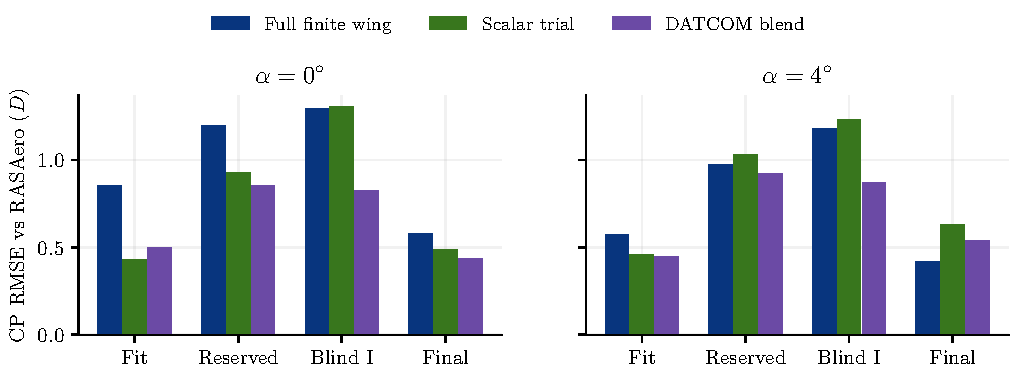
\includegraphics[width=.87\linewidth,height=.59\textheight,keepaspectratio]{figures/transfer-tests.pdf}
\begin{columns}[T,onlytextwidth]
\column{.49\textwidth}\small\textbf{Final three, $0^\circ$:} 0.58 to 0.44 $D$ RMS. The strongest improvement is on the highly tapered rocket.
\column{.48\textwidth}\small\textbf{Counterexample:} at $4^\circ$ the final group goes from 0.42 to 0.54 $D$ RMS. The near-rectangular rocket also worsens at $0^\circ$.
\end{columns}
\end{frame}
\begin{frame}{Iris: lower error through the burn, but the minimum is still early}
\begin{columns}[c,onlytextwidth]
\column{.68\textwidth}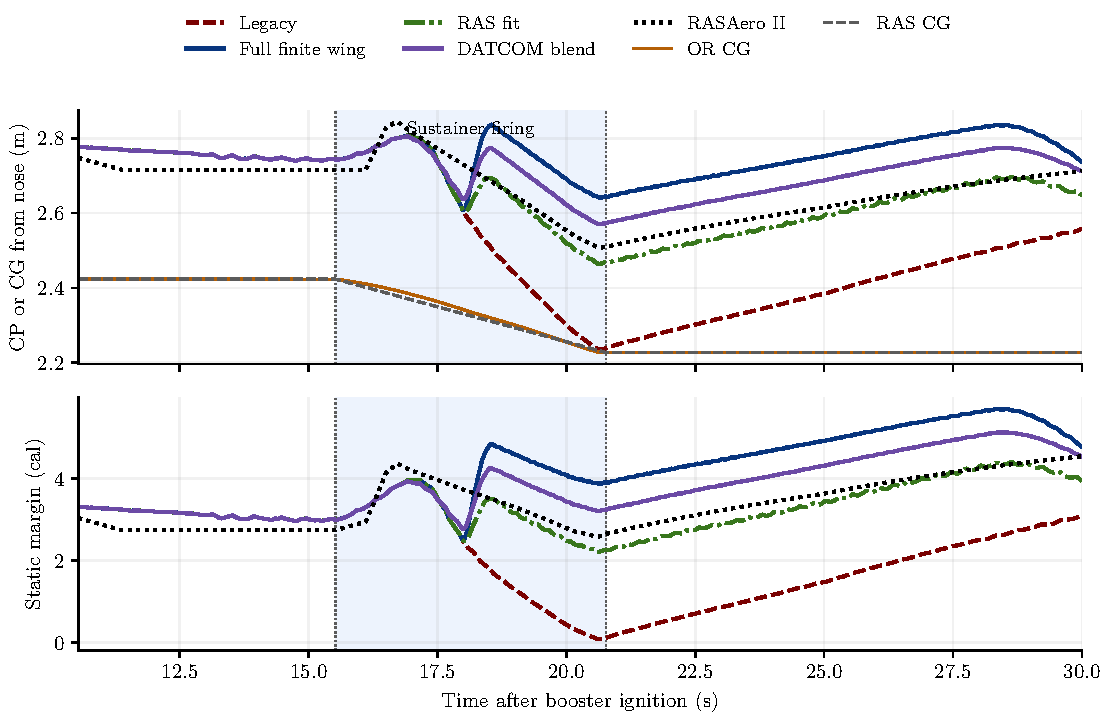
\includegraphics[width=\linewidth]{figures/iris-flight.pdf}
\column{.29\textwidth}\small
\textbf{Burn-wide margin RMS}\\Full: 0.95 cal\\DATCOM blend: 0.56 cal\\[.8em]
\textbf{Minimum margin}\\Blend: 2.77 cal at 18.00 s\\RASAero: 2.58 cal at 20.60 s\\[.8em]
At the same Mach, angle and stage, the blend still places CP 0.68 $D$ aft on average above Mach 2 in the sampled sustainer segment.
\end{columns}
\end{frame}
\begin{frame}{Use the blend for sensitivity studies; preserve both baselines}
\begin{columns}[T,onlytextwidth]
\column{.52\textwidth}
\begin{block}{Physical regression checks}
\small CP RMS in body diameters; five supersonic measurements per vehicle.\\[.5em]
\centering\begin{tabular}{lrr}\toprule
& ARCAS & Yuska B\\\midrule
Legacy & 2.665 & 1.023\\
Full & .318 & .126\\
Scalar & 1.047 & .511\\
DATCOM blend & .312 & .136\\\bottomrule\end{tabular}
\end{block}
\column{.44\textwidth}\small
\textbf{Scope.} The tunnel benchmarks constrain the blend. They are not independent evidence of its physical accuracy. ARCAS pitching-moment error increases despite nearly unchanged CP RMS.\\[.7em]
\textbf{Next measurement.} A matched bare/winged supersonic dataset with independent force and moment can separate forebody loading from wing--body interaction. Iris's Haack nose is currently represented by an ogive-chart surrogate.
\end{columns}
\end{frame}
\end{document}
